
%Copyright (C) 2016 by Krishneel@JSK Lab, The University of Tokyo

\documentclass{standalone}
\begin{document}

\subsection{Hardware}

We developed a hexarotor UAV as shown in Fig.\ref{fig:task1-uav}. As descrbied in  Fig.\ref{fig:task1-uav-platform}, this aerial robot consists of onboard sensors such as IMU, barometer, laser sensor, GPS for basic hovering flight control, as well as an original flight controller and a high level processor. The monocular camera is installed for egomotion estimation. The total weight of the UAV is 4.3 kg, while the flight time can reach 20 min with heavy vision processing on the onboard processor. We have achieved outdoor flight with autonomous altitude hold mode using our original sensor fusion algorithm (Fig.\ref{fig:task1-outdoor-flight}).

\begin{figure}[h]
  \begin{center}
    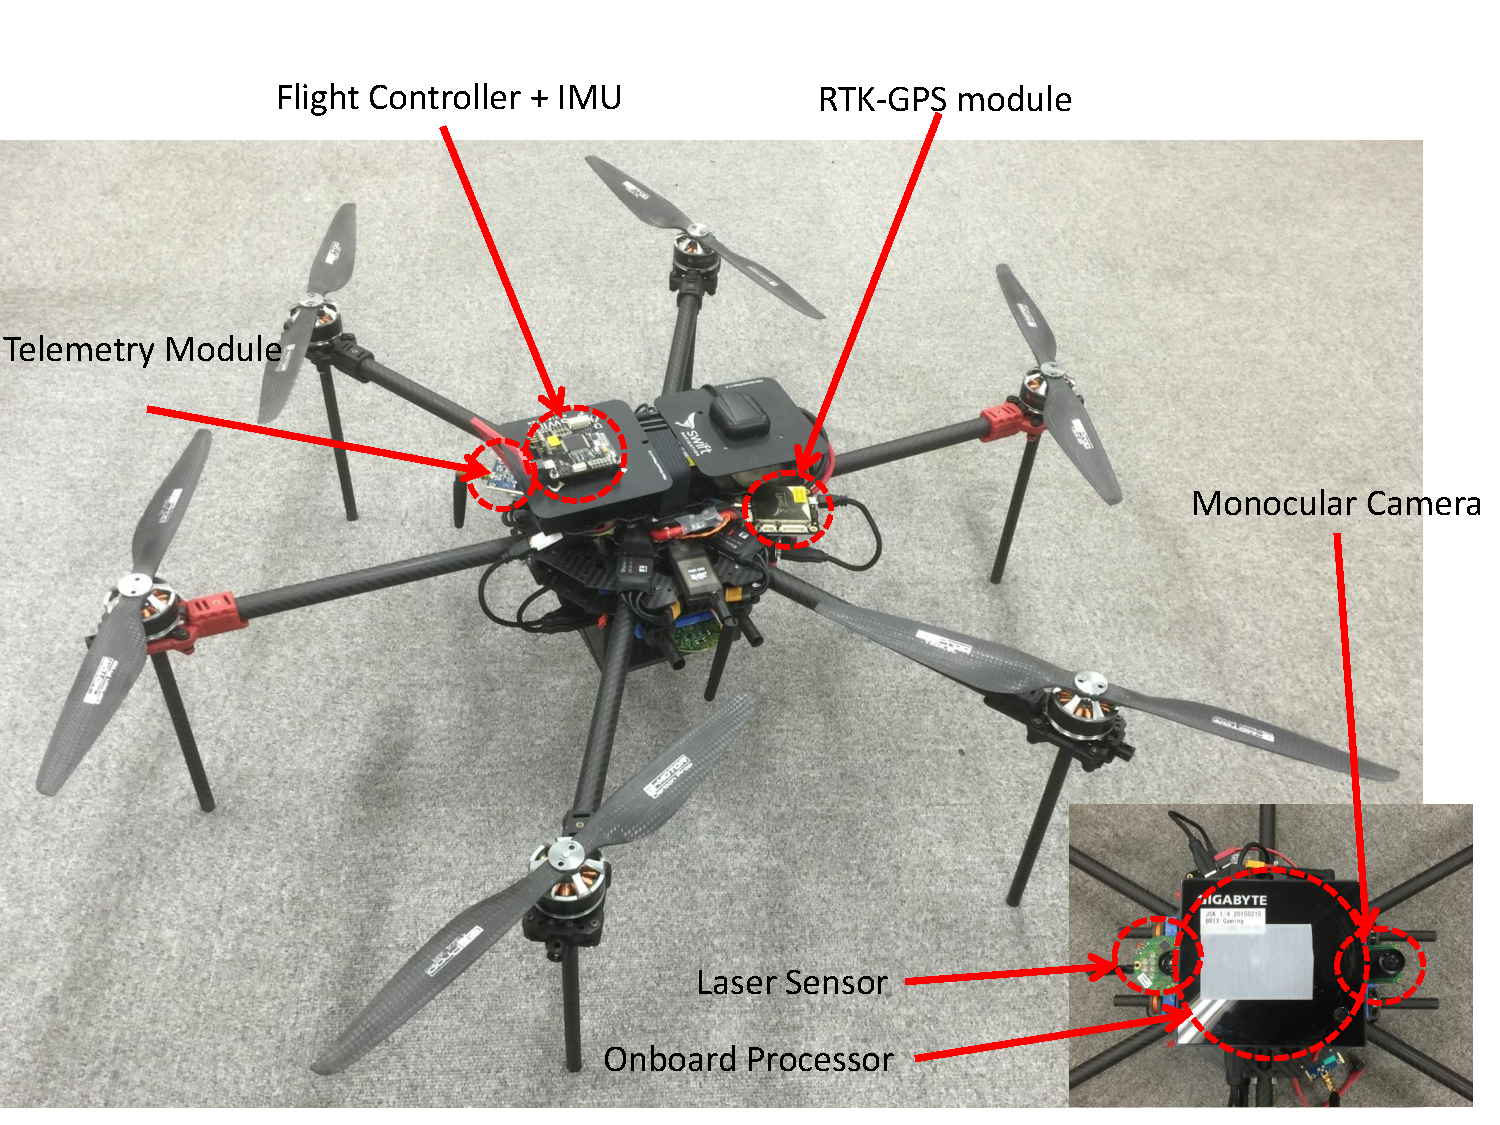
\includegraphics[clip,  bb=0 0 710 502,  width=\columnwidth]{sections/task1/images/task1-tarrot680.pdf}
    \caption{Image of task 1 UAV (Hawk)}
    \label{fig:task1-uav}
  \end{center}
\end{figure} 

\begin{figure}[h]
  \begin{center}
    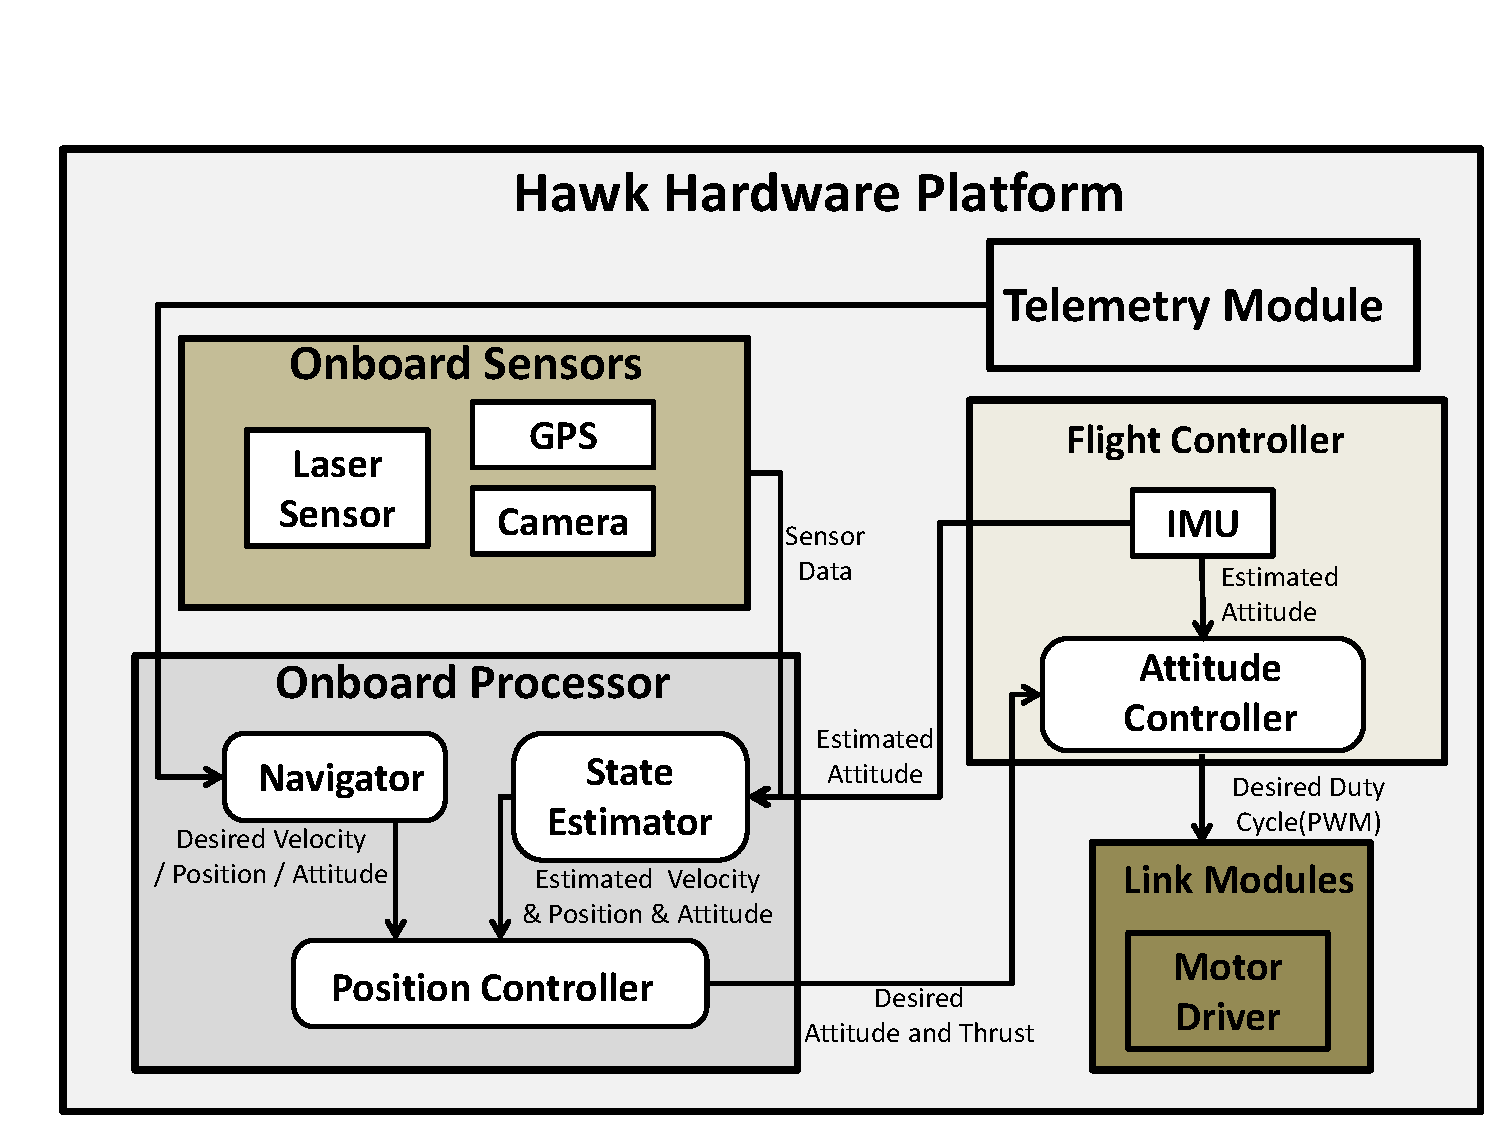
\includegraphics[clip,  bb=0 0 720 500,  width=\columnwidth]{sections/task1/images/hawk-platform.pdf}
    \caption{Hardware platform of Hawk}
    \label{fig:task1-uav-platform}
  \end{center}
\end{figure} 

\begin{figure}[h]
  \begin{center}
    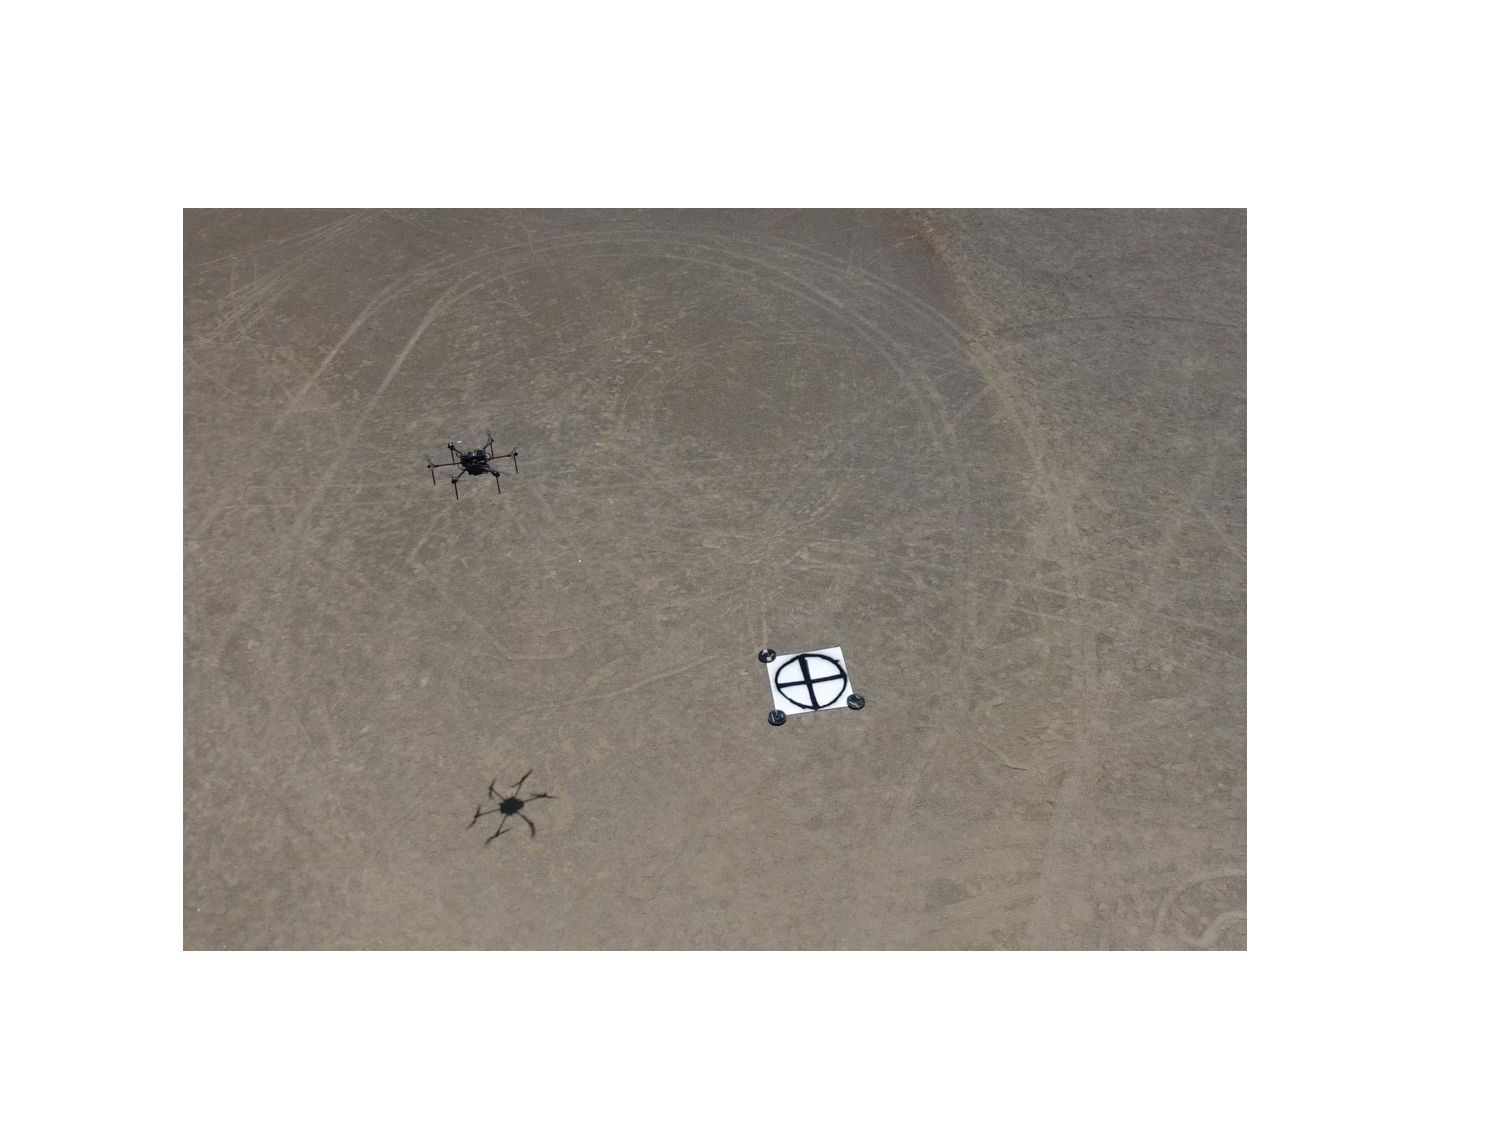
\includegraphics[clip,  bb=88 84 599 440,  width=\columnwidth]{sections/task1/images/task1-outdoor.pdf}
    \caption{Image of outdoor flight }
    \label{fig:task1-outdoor-flight}
  \end{center}
\end{figure} 



\end{document}
